% Generated by pysimcount.pfgroupfigure -- do not edit; regenerate instead.
% source: results/np-grouping/aggregate.json (seeds [1, 2, 3, 4, 5, 6, 7, 8, 9, 10]); run commits: 01d3c275ceae2840002bd1aaea68f59b987c4975
% formulas: suzuki2, suzuki4, mo-q14; groupings: xyz vs twogroup-even-out
% y: measured r, median over seeds; error bars: min and max over seeds
% figure made at git_commit=e42ff29056ad9ea7fc7c9899fab334903e42e3e3 git_dirty=True
% WARNING: the figure was made from uncommitted code; the commit above does not reproduce it.
% x is dodged for readability: X-Y-Z at n/1.025, two-group at n*1.025.
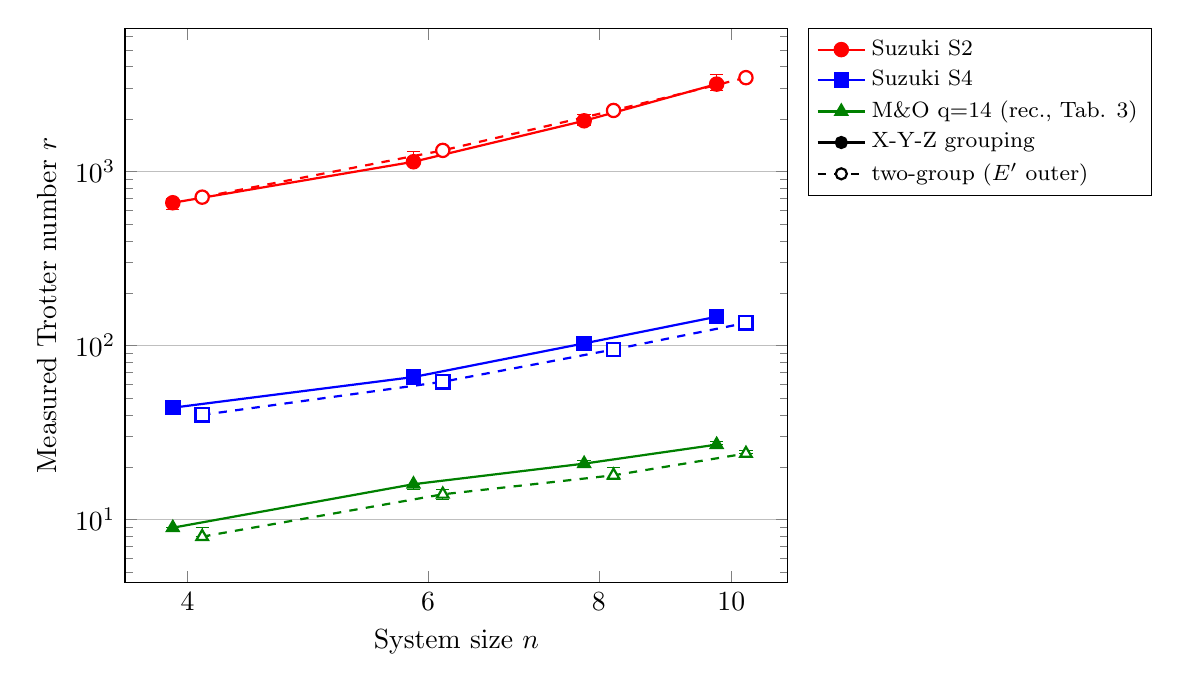
\begin{tikzpicture}
  \begin{loglogaxis}[
    width=10cm,
    xlabel={System size $n$},
    ylabel={Measured Trotter number $r$},
    xtick={4,6,8,10},
    xticklabels={4,6,8,10},
    xmin=3.6, xmax=11,
    ymajorgrids=true,
    legend pos=outer north east,
    legend cell align=left,
    legend style={font=\footnotesize},
  ]
    % suzuki2, xyz: (n, median r) with error bars to min and max over seeds
    \addplot[red, solid, thick, mark=*, mark size=2.4pt, mark options={solid, fill=red}, error bars/.cd, y dir=both, y explicit, error bar style={solid}] coordinates {
      (3.9024,661.5) += (0,37.5) -= (0,57.5)
      (5.8537,1137.5) += (0,170.5) -= (0,52.5)
      (7.8049,1955.5) += (0,167.5) -= (0,104.5)
      (9.7561,3176.5) += (0,433.5) -= (0,264.5)
    };
    \addlegendentry{Suzuki S2}
    % suzuki2, twogroup-even-out: (n, median r) with error bars to min and max over seeds
    \addplot[red, dashed, thick, mark=*, mark size=2.4pt, mark options={solid, fill=white}, forget plot, error bars/.cd, y dir=both, y explicit, error bar style={solid}] coordinates {
      (4.1000,712.5) += (0,6.5) -= (0,5.5)
      (6.1500,1322) += (0,16) -= (0,5)
      (8.2000,2241.5) += (0,26.5) -= (0,21.5)
      (10.2500,3459.5) += (0,134.5) -= (0,64.5)
    };
    % suzuki4, xyz: (n, median r) with error bars to min and max over seeds
    \addplot[blue, solid, thick, mark=square*, mark size=2.4pt, mark options={solid, fill=blue}, error bars/.cd, y dir=both, y explicit, error bar style={solid}] coordinates {
      (3.9024,44) += (0,1) -= (0,0)
      (5.8537,66) += (0,5) -= (0,3)
      (7.8049,103) += (0,4) -= (0,4)
      (9.7561,146.5) += (0,13.5) -= (0,3.5)
    };
    \addlegendentry{Suzuki S4}
    % suzuki4, twogroup-even-out: (n, median r) with error bars to min and max over seeds
    \addplot[blue, dashed, thick, mark=square*, mark size=2.4pt, mark options={solid, fill=white}, forget plot, error bars/.cd, y dir=both, y explicit, error bar style={solid}] coordinates {
      (4.1000,40) += (0,1) -= (0,1)
      (6.1500,62) += (0,1) -= (0,0)
      (8.2000,95) += (0,1) -= (0,1)
      (10.2500,135) += (0,3) -= (0,1)
    };
    % mo-q14, xyz: (n, median r) with error bars to min and max over seeds
    \addplot[green!50!black, solid, thick, mark=triangle*, mark size=2.4pt, mark options={solid, fill=green!50!black}, error bars/.cd, y dir=both, y explicit, error bar style={solid}] coordinates {
      (3.9024,9) += (0,0) -= (0,0)
      (5.8537,16) += (0,0) -= (0,1)
      (7.8049,21) += (0,1) -= (0,1)
      (9.7561,27) += (0,1) -= (0,0)
    };
    \addlegendentry{M\&O q=14 (rec., Tab. 3)}
    % mo-q14, twogroup-even-out: (n, median r) with error bars to min and max over seeds
    \addplot[green!50!black, dashed, thick, mark=triangle*, mark size=2.4pt, mark options={solid, fill=white}, forget plot, error bars/.cd, y dir=both, y explicit, error bar style={solid}] coordinates {
      (4.1000,8) += (0,1) -= (0,0)
      (6.1500,14) += (0,1) -= (0,1)
      (8.2000,18) += (0,2) -= (0,1)
      (10.2500,24) += (0,1) -= (0,0)
    };
    \addlegendimage{black, solid, thick, mark=*, mark options={solid, fill=black}}
    \addlegendentry{X-Y-Z grouping}
    \addlegendimage{black, dashed, thick, mark=*, mark options={solid, fill=white}}
    \addlegendentry{two-group ($E'$ outer)}
  \end{loglogaxis}
\end{tikzpicture}
